\documentclass[12pt]{article}

% ── Geometry ──────────────────────────────────────────────────────────────────
\usepackage[a4paper, margin=2.5cm]{geometry}

% ── Fonts & encoding ─────────────────────────────────────────────────────────
\usepackage[T1]{fontenc}
\usepackage[utf8]{inputenc}
\usepackage{lmodern}
\usepackage{microtype}

% ── Math ──────────────────────────────────────────────────────────────────────
\usepackage{amsmath, amssymb, mathtools}

% ── Tables ────────────────────────────────────────────────────────────────────
\usepackage{booktabs}
\usepackage{array}
\usepackage{multirow}
\usepackage{tabularx}

% ── Graphics ──────────────────────────────────────────────────────────────────
\usepackage{graphicx}
\usepackage{float}
\usepackage{tikz}
\usetikzlibrary{arrows.meta, positioning, shapes.geometric, calc, fit}

% ── Code listings ─────────────────────────────────────────────────────────────
\usepackage{listings}
\lstset{
  basicstyle=\ttfamily\small,
  breaklines=true,
  frame=single,
  numbers=none,
  captionpos=b,
  aboveskip=8pt,
  belowskip=8pt,
  xleftmargin=4pt,
  xrightmargin=4pt,
}
\lstdefinelanguage{Solidity}{
  keywords={function, external, view, pure, returns, uint256, address, string, memory, interface, contract, modifier, require, emit, event, mapping, bool, internal, override, public, private},
  keywordstyle=\bfseries,
  sensitive=true,
  comment=[l]{//},
  morecomment=[s]{/*}{*/},
  string=[b]",
}

% ── Hyperlinks ────────────────────────────────────────────────────────────────
\usepackage[colorlinks=true, linkcolor=blue!60!black, citecolor=blue!60!black, urlcolor=blue!70!black]{hyperref}

% ── Bibliography ──────────────────────────────────────────────────────────────
\usepackage[numbers,sort&compress]{natbib}

% ── Misc ──────────────────────────────────────────────────────────────────────
\usepackage{enumitem}
\usepackage{xcolor}
\usepackage{caption}
\captionsetup{font=small, labelfont=bf}

% ══════════════════════════════════════════════════════════════════════════════
\begin{document}

% ── Title block ───────────────────────────────────────────────────────────────
\begin{center}
  {\LARGE\bfseries AI-Managed ERC-4626 Yield Vault\\[4pt]
   with Multi-Criteria Decision Making:\\[4pt]
   Design, Implementation, and Formal Verification}

  \bigskip

  Solovev Sergei\\
  Faculty of Computer Science, HSE University, Moscow, Russia

  \medskip

  \texttt{sesesolovev@edu.hse.ru}
  \quad$\cdot$\quad
  \url{https://sergeisolovev.com}

  \smallskip

  Code: \url{https://github.com/[REDACTED]}

  \medskip

  April 15, 2026
\end{center}

\bigskip

% ── Abstract ──────────────────────────────────────────────────────────────────
\begin{center}
  \textbf{Abstract}
\end{center}
\begin{quote}
We present a novel approach to automated DeFi yield optimisation through an agent-managed ERC-4626 tokenised vault.
The system employs a hybrid off-chain/on-chain architecture where a Python-based AI agent applies Multi-Criteria Decision Making (MCDM) with weighted scoring across four factors---yield, risk, cost-efficiency, and stability---to autonomously rebalance user deposits between Aave~V3 and Compound~V3 lending protocols.
Unlike existing yield optimisers that rely on simple APY comparison, our agent produces cryptographically signed decisions using EIP-712 typed data, enabling on-chain verification of every rebalance while maintaining the computational flexibility of off-chain analysis.
The system achieves formal safety guarantees through invariant testing with 76{,}800+ randomised function calls and zero violations, and includes a Chainlink Automation fallback for protocol liveness.
We deploy and validate the system on Ethereum Sepolia testnet with USDC as the underlying asset.

\medskip
\noindent\textbf{Keywords:} DeFi, yield optimisation, ERC-4626, EIP-712, multi-criteria decision making, smart contracts, Ethereum, Solidity, agent-based systems
\end{quote}

% ══════════════════════════════════════════════════════════════════════════════
\section{Introduction}

\subsection{Decentralised Finance: A Primer}

Decentralised Finance (DeFi) refers to a class of financial applications built on public blockchains---primarily Ethereum---that replicate traditional financial services (lending, borrowing, trading, insurance) without centralised intermediaries.
Instead of banks, DeFi protocols use \emph{smart contracts}: self-executing programs deployed on the blockchain that enforce rules automatically and transparently.

As of early 2026, the total value locked (TVL) in DeFi protocols exceeds \$180~billion, with lending protocols comprising approximately 40\% of this figure~\cite{defillama}.

\subsection{Lending Protocols}

DeFi lending protocols allow users to \emph{supply} assets to earn interest (supply-side yield) or \emph{borrow} assets against collateral (demand-side).
The interest rate is determined algorithmically based on \emph{utilisation}---the ratio of borrowed assets to supplied assets:
\begin{equation}
  U = \frac{\text{Total Borrowed}}{\text{Total Supplied}}
  \label{eq:utilisation}
\end{equation}
Higher utilisation means more demand for borrowing, which increases the supply rate (APY earned by depositors) and the borrow rate (cost paid by borrowers).

Two dominant lending protocols on Ethereum are:

\textbf{Aave~V3}~\cite{aave}---the largest lending protocol by TVL.
Key characteristics: variable and stable borrow rates, cross-chain liquidity via portals, risk-isolated markets (E-mode), and rates stored in \emph{RAY} format ($1\;\text{RAY} = 10^{27}$), already annualised.

\textbf{Compound~V3 (Comet)}~\cite{compound}---a streamlined single-asset lending market:
one base asset per market (e.g., USDC), per-second interest accrual, rates returned as per-second values requiring annualisation, and built-in multi-collateral support.

\subsection{The Yield Optimisation Problem}

Supply rates on lending protocols are \emph{volatile}.
They fluctuate based on market-wide borrowing demand, protocol governance parameters, token incentive programmes, and macro events affecting crypto markets.
Figure~\ref{fig:rate-crossover} illustrates a typical scenario where Aave and Compound supply rates cross over time, creating opportunities for optimisation.

\begin{figure}[H]
\centering
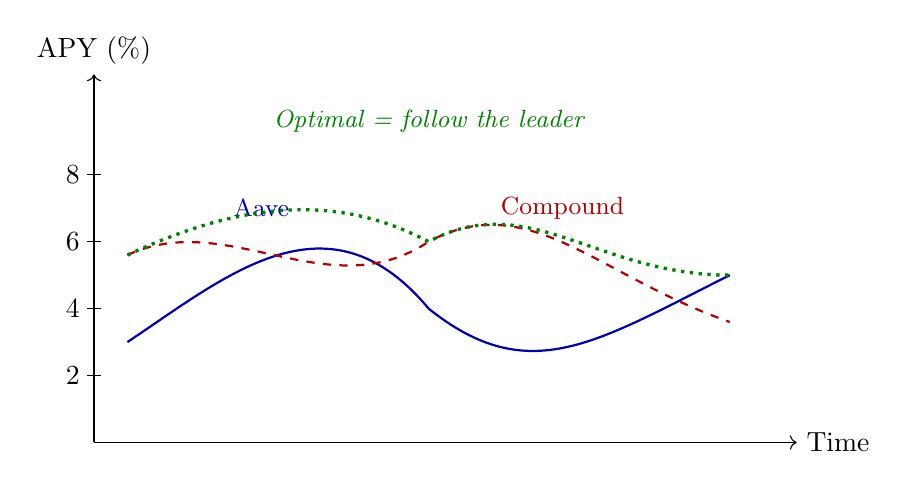
\begin{tikzpicture}[scale=0.85]
  \draw[->] (0,0) -- (10.5,0) node[right] {Time};
  \draw[->] (0,0) -- (0,5.5) node[above] {APY (\%)};
  \foreach \y/\l in {1/2, 2/4, 3/6, 4/8} {
    \draw (-0.1,\y) -- (0.1,\y) node[left=4pt] {\l};
  }
  % Aave line
  \draw[blue!70!black, thick] (0.5,1.5) .. controls (2,2.5) and (3.5,3.8) ..
    (5,2) .. controls (6.5,0.8) and (7.5,1.5) .. (9.5,2.5);
  \node[blue!70!black, font=\small] at (2.5,3.5) {Aave};
  % Compound line
  \draw[red!70!black, thick, dashed] (0.5,2.8) .. controls (2,3.5) and (3.5,2) ..
    (5,3) .. controls (6.5,3.8) and (7.5,2.5) .. (9.5,1.8);
  \node[red!70!black, font=\small] at (7,3.5) {Compound};
  % Optimal region
  \draw[green!50!black, very thick, dotted] (0.5,2.8) .. controls (2,3.5) and (3.5,3.8) ..
    (5,3) .. controls (6.5,3.8) and (7.5,2.5) .. (9.5,2.5);
  \node[green!50!black, font=\small\itshape] at (5,4.8) {Optimal = follow the leader};
\end{tikzpicture}
\caption{DeFi lending rate crossover.  Rates change every block ($\sim$12~s).
The optimal strategy follows the highest rate, but gas costs, timing risk, and utilisation must be considered.}
\label{fig:rate-crossover}
\end{figure}

A rational depositor should always hold funds in the protocol offering the highest risk-adjusted return.
However, \emph{manual optimisation is impractical} because:
\begin{enumerate}[nosep]
  \item \textbf{Monitoring cost}: rates change every block ($\sim$12~seconds on Ethereum).
  \item \textbf{Transaction cost}: each rebalance requires gas (\$2--50 depending on network conditions).
  \item \textbf{Complexity}: raw APY is an incomplete signal---utilisation risk, rate stability, and switching costs all matter.
  \item \textbf{Timing}: rebalancing at the wrong time (e.g., during a temporary rate spike) destroys value.
\end{enumerate}

\subsection{Limitations of Existing Solutions}

Existing yield optimisers fall into two architectural categories, each with fundamental limitations (Table~\ref{tab:existing-limitations}).

\begin{table}[H]
\centering
\caption{Architectural trade-offs in existing yield optimisers.}
\label{tab:existing-limitations}
\small
\begin{tabular}{@{}lll@{}}
\toprule
 & \textbf{On-Chain Only} & \textbf{Off-Chain Opaque} \\
\midrule
Examples       & Yearn~V3, Beefy, Idle Finance & Almanak \\
Decision logic & Simple threshold           & ML models (proprietary) \\
Strengths      & Fully transparent, trustless & Complex analysis possible \\
Weaknesses     & Cannot compute multi-factor  & Users trust a black box; \\
               & analysis (gas-prohibitive)   & no on-chain proof \\
Verifiability  & Full (but limited logic)     & None \\
\bottomrule
\end{tabular}
\end{table}

\subsection{Our Contribution}

We propose a \emph{hybrid architecture} that combines the computational power of off-chain analysis with the trustless verification of on-chain execution.
Our contributions are:

\begin{enumerate}[nosep]
  \item \textbf{Multi-Criteria Decision Making (MCDM)}: a weighted scoring model across four factors (APY, risk, cost, stability) rather than single-factor APY comparison (Section~\ref{sec:mcdm}).
  \item \textbf{Cryptographic decision verification}: every agent decision is signed with EIP-712 typed data and verified on-chain, creating an auditable trail (Section~\ref{sec:eip712}).
  \item \textbf{Formal safety guarantees}: invariant testing with stateful fuzzing proves vault solvency under arbitrary operation sequences (Section~\ref{sec:testing}).
  \item \textbf{Graceful degradation}: Chainlink Automation fallback ensures the vault is never unmanaged if the agent goes offline (Section~\ref{sec:chainlink}).
  \item \textbf{Natural language interface}: integration with OpenClaw chat framework enables conversational interaction with the vault (Section~\ref{sec:openclaw}).
\end{enumerate}

% ══════════════════════════════════════════════════════════════════════════════
\section{Background}

\subsection{ERC-4626: Tokenised Vault Standard}

ERC-4626~\cite{eip4626} is an Ethereum standard for tokenised vaults.
It extends ERC-20 (fungible token) with standardised deposit/withdraw mechanics.

\textbf{Core invariant:} a user's claim on the vault's underlying assets is proportional to their share of the total supply.
The share price is:
\begin{equation}
  p = \frac{\text{totalAssets}}{\text{totalSupply}}
  \label{eq:share-price}
\end{equation}
When a user deposits $a$ assets into a vault with total assets $A$ and total supply $S$, they receive shares:
\begin{equation}
  s = \left\lfloor \frac{a \cdot (S + 10^d)}{A + 1} \right\rfloor
  \label{eq:deposit-shares}
\end{equation}
where $d$ is the \emph{decimals offset} (a protection parameter explained in Section~\ref{sec:inflation}).
The floor function reflects Solidity's integer division, which always rounds towards zero.

When redeeming $s$ shares:
\begin{equation}
  a = \left\lfloor \frac{s \cdot (A + 1)}{S + 10^d} \right\rfloor
  \label{eq:redeem-assets}
\end{equation}

\textbf{Key property:} the conversion always rounds in favour of the vault (down for deposits, down for withdrawals), preventing rounding-based exploits.

\subsection{UUPS Proxy Pattern}

Smart contracts on Ethereum are \emph{immutable} once deployed.
The Universal Upgradeable Proxy Standard (UUPS, ERC-1967)~\cite{erc1967} enables upgradeability by separating storage (in a proxy contract) from logic (in an implementation contract):
\[
  \text{User} \;\to\; \text{Proxy (storage)} \;\xrightarrow{\texttt{delegatecall}}\; \text{Implementation (logic)}
\]
This allows fixing bugs, adding features, or upgrading dependencies without migrating user funds.

\subsection{EIP-712: Typed Structured Data Signing}
\label{sec:eip712}

EIP-712~\cite{eip712} defines a standard for signing structured data (not just raw bytes).
This enables human-readable signing, domain binding (signatures include the contract address and chain ID, preventing cross-chain replay), and type safety.

The signing process produces a digest:
\begin{equation}
  \text{digest} = \text{keccak256}\!\big(\texttt{0x1901} \;\|\; \text{domainSeparator} \;\|\; \text{structHash}\big)
  \label{eq:eip712-digest}
\end{equation}
where:
\begin{align}
  \text{domainSeparator} &= \text{keccak256}\!\big(\text{encode}(\text{typeHash}_{\text{dom}},\, \text{name},\, \text{version},\, \text{chainId},\, \text{contract})\big) \label{eq:domain-sep} \\[4pt]
  \text{structHash} &= \text{keccak256}\!\big(\text{encode}(\text{typeHash}_{\text{params}},\, \text{target},\, \text{maxLoss},\, \text{ts},\, \text{nonce})\big) \label{eq:struct-hash}
\end{align}
The agent signs this digest with its private key, producing $(v, r, s)$.
The vault recovers the signer using \texttt{ecrecover} and verifies it matches the authorised keeper.

\subsection{Exponential Moving Average}

An Exponential Moving Average (EMA) is a weighted average that gives more weight to recent observations:
\begin{equation}
  S_t = \alpha \cdot X_t + (1 - \alpha) \cdot S_{t-1}, \quad \alpha \in (0, 1]
  \label{eq:ema}
\end{equation}
where $\alpha$ is the smoothing factor.
Higher $\alpha$ means faster response to new data but more sensitivity to noise.

Properties:
\begin{itemize}[nosep]
  \item \textbf{Memory}: EMA implicitly considers all past observations with exponentially decaying weights.
  \item \textbf{Lag}: EMA lags behind the true signal by approximately $\frac{1-\alpha}{\alpha}$ periods.
  \item \textbf{Smoothing}: random spikes are dampened by factor $(1-\alpha)$.
\end{itemize}
We use $\alpha = 0.3$, meaning each new rate observation has 30\% influence on the smoothed value.

% ══════════════════════════════════════════════════════════════════════════════
\section{System Architecture}

\subsection{Overview}

The system consists of three layers (Figure~\ref{fig:architecture}).

\begin{figure}[H]
\centering
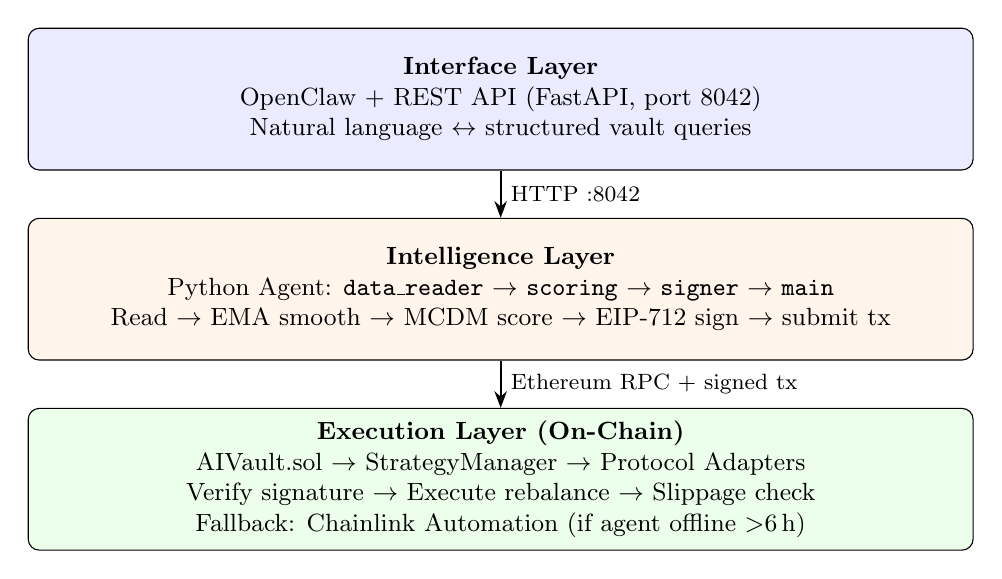
\begin{tikzpicture}[
  layer/.style={draw, rounded corners=4pt, minimum width=12cm, minimum height=1.8cm, align=center, font=\small},
  arr/.style={-{Stealth[length=6pt]}, thick},
  node distance=0.6cm
]
  \node[layer, fill=blue!8] (iface)
    {\textbf{Interface Layer}\\OpenClaw + REST API (FastAPI, port 8042)\\Natural language $\leftrightarrow$ structured vault queries};
  \node[layer, fill=orange!8, below=of iface] (intel)
    {\textbf{Intelligence Layer}\\Python Agent: \texttt{data\_reader} $\to$ \texttt{scoring} $\to$ \texttt{signer} $\to$ \texttt{main}\\Read $\to$ EMA smooth $\to$ MCDM score $\to$ EIP-712 sign $\to$ submit tx};
  \node[layer, fill=green!8, below=of intel] (exec)
    {\textbf{Execution Layer (On-Chain)}\\AIVault.sol $\to$ StrategyManager $\to$ Protocol Adapters\\Verify signature $\to$ Execute rebalance $\to$ Slippage check\\Fallback: Chainlink Automation (if agent offline $>$6\,h)};

  \draw[arr] (iface) -- node[right, font=\footnotesize] {HTTP :8042} (intel);
  \draw[arr] (intel) -- node[right, font=\footnotesize] {Ethereum RPC + signed tx} (exec);
\end{tikzpicture}
\caption{Three-layer system architecture.  The interface layer provides natural language access; the intelligence layer performs off-chain MCDM scoring and EIP-712 signing; the execution layer verifies and executes on-chain.}
\label{fig:architecture}
\end{figure}

\subsection{Adapter Pattern (Strategy Design Pattern)}

To support multiple lending protocols with a single vault, we employ the Strategy design pattern~\cite{gof} through the \texttt{IProtocolAdapter} interface:

\begin{lstlisting}[language=Solidity]
interface IProtocolAdapter {
    function supply(address asset, uint256 amount) external;
    function withdraw(address asset, uint256 amount) external returns (uint256);
    function balance(address asset) external view returns (uint256);
    function getSupplyRate(address asset) external view returns (uint256);
    function getUtilization(address asset) external view returns (uint256);
    function protocolName() external pure returns (string memory);
}
\end{lstlisting}

Each protocol adapter implements this interface with protocol-specific logic (Table~\ref{tab:adapter-ops}).

\begin{table}[H]
\centering
\caption{Protocol adapter operation mapping.}
\label{tab:adapter-ops}
\small
\begin{tabular}{@{}lll@{}}
\toprule
\textbf{Operation} & \textbf{Aave~V3} & \textbf{Compound~V3} \\
\midrule
\texttt{supply}       & \texttt{pool.supply(asset, amt, self, 0)} & \texttt{comet.supply(asset, amt)} \\
\texttt{withdraw}     & \texttt{pool.withdraw(asset, amt, to)}    & \texttt{comet.withdraw(asset, amt)} \\
\texttt{balance}      & \texttt{aToken.balanceOf(this)}           & \texttt{comet.balanceOf(this)} \\
\texttt{getSupplyRate}& $\texttt{liquidityRate}_{\text{RAY}}/10^9$& $r_{\text{sec}} \times T_{\text{year}}$ \\
\bottomrule
\end{tabular}
\end{table}

\textbf{Extensibility:} adding a new protocol (e.g., Morpho, Euler) requires only implementing a new adapter---no changes to the vault or strategy manager.

\subsection{Contract Inheritance Graph}

The vault contract inherits from six OpenZeppelin upgradeable base contracts:

\begin{figure}[H]
\centering
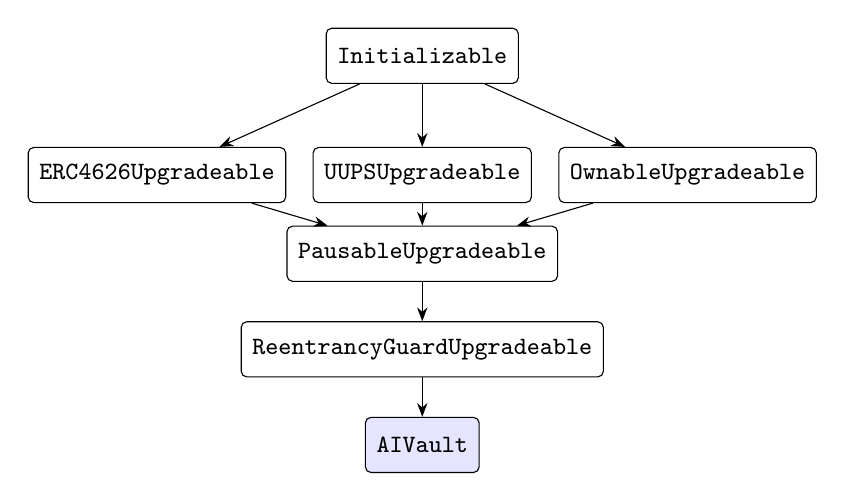
\begin{tikzpicture}[
  box/.style={draw, rounded corners=2pt, font=\small\ttfamily, minimum height=0.7cm, inner sep=4pt},
  arr/.style={-{Stealth[length=5pt]}},
  node distance=0.5cm and 0.3cm
]
  \node[box] (init) {Initializable};
  \node[box, below left=0.8cm and 0.5cm of init] (erc) {ERC4626Upgradeable};
  \node[box, below=0.8cm of init] (uups) {UUPSUpgradeable};
  \node[box, below right=0.8cm and 0.5cm of init] (own) {OwnableUpgradeable};
  \node[box, below=1.8cm of init] (pause) {PausableUpgradeable};
  \node[box, below=0.5cm of pause] (reen) {ReentrancyGuardUpgradeable};
  \node[box, fill=blue!10, below=0.5cm of reen] (vault) {\textbf{AIVault}};

  \draw[arr] (init) -- (erc);
  \draw[arr] (init) -- (uups);
  \draw[arr] (init) -- (own);
  \draw[arr] (erc) -- (pause);
  \draw[arr] (uups) -- (pause);
  \draw[arr] (own) -- (pause);
  \draw[arr] (pause) -- (reen);
  \draw[arr] (reen) -- (vault);
\end{tikzpicture}
\caption{AIVault contract inheritance hierarchy.}
\label{fig:inheritance}
\end{figure}

\subsection{Fund Flow}

Deposits, withdrawals, and rebalances follow well-defined paths:

\begin{itemize}[nosep]
  \item \textbf{Deposit}: User $\xrightarrow{\text{USDC}}$ Vault (idle) $\xrightarrow{\text{deploy}}$ Active Adapter $\xrightarrow{\text{supply}}$ Protocol
  \item \textbf{Withdraw}: User $\xleftarrow{\text{USDC}}$ Vault (idle) $\xleftarrow{\text{unwind}}$ Active Adapter $\xleftarrow{\text{withdraw}}$ Protocol
  \item \textbf{Rebalance}: Adapter$_A$ $\xrightarrow{\text{withdraw}}$ Vault (idle) $\xrightarrow{\text{supply}}$ Adapter$_B$
\end{itemize}

The vault maintains an \emph{idle buffer} ($b = 2\%$ of TVL) to serve small withdrawals without touching the protocol, reducing gas costs for users.

% ══════════════════════════════════════════════════════════════════════════════
\section{Mathematical Foundations}

\subsection{ERC-4626 Inflation Attack and Mitigation}
\label{sec:inflation}

\textbf{The attack}~\cite{oz-inflation}: an attacker can steal a victim's deposit through share price manipulation:
\begin{enumerate}[nosep]
  \item Attacker deposits 1~wei, receiving 1~share.
  \item Attacker ``donates'' $D$ tokens directly to the vault (no deposit, just transfer).
  \item Now: $\text{totalAssets} = D + 1$, $\text{totalSupply} = 1$.
  \item Victim deposits $V$ tokens, receiving shares: $s = \lfloor V \cdot 1 / (D + 1) \rfloor$.
  \item If $D \geq V$, the victim receives \textbf{0~shares} and loses their deposit.
\end{enumerate}

\textbf{Our mitigation:} we set \texttt{\_decimalsOffset() = 6}, which creates $10^6$ virtual shares in the conversion formula:
\begin{equation}
  s = \left\lfloor \frac{a \cdot (S + 10^6)}{A + 1} \right\rfloor
  \label{eq:virtual-shares}
\end{equation}
For the attack to succeed with offset $d = 6$:
\begin{equation}
  D \geq V \cdot 10^6
  \label{eq:attack-cost}
\end{equation}
To steal a 10{,}000~USDC deposit, the attacker would need to donate $10^{10}$~USDC (\$10~billion), making the attack economically infeasible.

\textbf{Formal verification:} our test \texttt{test\_inflationAttack\_mitigated} confirms that after a 10{,}000~USDC donation, a victim depositing 10{,}000~USDC still receives shares worth $\approx$\,10{,}000~USDC (within 1\% tolerance).

\subsection{APY Normalisation}

Different protocols represent interest rates in incompatible formats.
We normalise all rates to a common \emph{annual, $10^{18}$-scaled} representation.

\textbf{Aave~V3:} rates are stored in RAY ($10^{27}$) and are already annualised:
\begin{equation}
  \text{APY}_{1e18} = \frac{\text{currentLiquidityRate}_{\text{RAY}}}{10^9}
  \label{eq:aave-norm}
\end{equation}
\emph{Example:} a 5\% APY in Aave $= 5 \times 10^{25}$ RAY $\to$ $5 \times 10^{16}$ in $10^{18}$~scale.

\textbf{Compound~V3:} rates are per-second and must be annualised:
\begin{equation}
  \text{APY}_{1e18} = r_{\text{sec}} \times T_{\text{year}}
  \label{eq:compound-norm}
\end{equation}
where $T_{\text{year}} = 365.25 \times 24 \times 3600 = 31\,557\,600$ seconds.

\emph{Example:} a per-second rate of $1.585 \times 10^{9}$ $\to$ $1.585 \times 10^{9} \times 3.156 \times 10^{7} \approx 5 \times 10^{16}$ (5\% APY).

\subsection{EMA Rate Smoothing}

Raw APY readings are noisy and susceptible to flash manipulation.
We apply EMA smoothing both on-chain (StrategyManager) and off-chain (agent):
\begin{equation}
  S_t = \alpha \cdot R_t + (1 - \alpha) \cdot S_{t-1}, \quad \alpha = 0.3
  \label{eq:ema-rate}
\end{equation}

\textbf{Rate manipulation guard:} on-chain, if the jump between the raw rate and the smoothed rate exceeds a threshold $J_{\max} = 500$~bps (5\%):
\begin{equation}
  \lvert R_t - S_{t-1} \rvert > J_{\max} \cdot 10^{14} \implies \text{skip update}
  \label{eq:jump-guard}
\end{equation}
This prevents an attacker from using flash loans to spike a protocol's utilisation and manipulate the agent's scoring.

\subsection{Multi-Criteria Decision Making (MCDM)}
\label{sec:mcdm}

The core innovation of our system is a \emph{weighted multi-factor scoring model} that evaluates each protocol across four dimensions.
Each factor $f_k$ is normalised to $[0, 1]$ and combined with weights $w_k$:
\begin{equation}
  \text{Score}_i = \sum_{k=1}^{4} w_k \cdot f_k(i) = 0.40\,f_{\text{APY}} + 0.25\,f_{\text{Risk}} + 0.20\,f_{\text{Cost}} + 0.15\,f_{\text{Stab}}
  \label{eq:mcdm}
\end{equation}

\subsubsection{Factor 1: APY Score ($w_1 = 0.40$)}

\begin{equation}
  f_{\text{APY}}(i) = \text{clamp}\!\left(\frac{\text{smoothedAPY}_i}{\text{APY}_{\max}},\; 0,\; 1\right)
  \label{eq:f-apy}
\end{equation}
where $\text{APY}_{\max} = 20\%$ is the normalisation ceiling.

\emph{Rationale:} yield is the primary objective, but not the only consideration.

\subsubsection{Factor 2: Risk Score ($w_2 = 0.25$)}

\begin{equation}
  f_{\text{Risk}}(i) = 1 - \text{clamp}(\text{utilisation}_i,\; 0,\; 1)
  \label{eq:f-risk}
\end{equation}

\emph{Rationale:} high utilisation ($U > 0.8$) signals increased probability of rate drop when borrowers repay, potential liquidity constraints for large withdrawals, and higher sensitivity to market shocks.
A protocol at 30\% utilisation scores $1 - 0.3 = 0.7$; one at 95\% utilisation scores only $0.05$.

\subsubsection{Factor 3: Cost Score ($w_3 = 0.20$)}

\begin{equation}
  f_{\text{Cost}}(i) = 1 - \text{clamp}\!\left(\frac{g \cdot G}{g_{\max}},\; 0,\; 1\right)
  \label{eq:f-cost}
\end{equation}
where $g$ is the gas price (wei), $G = 200\,000$ is the estimated rebalance gas, and $g_{\max} = 0.01$~ETH is the normalisation ceiling.

\emph{Rationale:} a rebalance is only worthwhile if the expected yield improvement exceeds the switching cost.

\subsubsection{Factor 4: Stability Score ($w_4 = 0.15$)}

\begin{equation}
  f_{\text{Stab}}(i) = 1 - \text{clamp}\!\left(\frac{\lvert\Delta\text{TVL}_i\rvert}{0.30},\; 0,\; 1\right)
  \label{eq:f-stab}
\end{equation}
where $\Delta\text{TVL}_i$ is the fractional TVL change since the last observation.

\emph{Rationale:} a protocol experiencing rapid TVL outflows may be at risk of liquidity crisis, rate instability, or protocol-specific issues.

\subsubsection{Decision Rule}

The agent rebalances when:
\begin{equation}
  \text{Score}_{\text{best}} - \text{Score}_{\text{current}} \geq \theta, \quad \theta = 0.05
  \label{eq:threshold}
\end{equation}
This hysteresis threshold prevents \emph{thrashing}---repeatedly switching between protocols with similar scores.

\subsubsection{Numerical Example}

Consider the market state in Table~\ref{tab:example-input}.

\begin{table}[H]
\centering
\caption{Example market state for MCDM scoring.}
\label{tab:example-input}
\small
\begin{tabular}{@{}lcccc@{}}
\toprule
\textbf{Protocol} & \textbf{APY} & \textbf{Utilisation} & \textbf{Gas (ETH)} & \textbf{TVL~$\Delta$} \\
\midrule
Aave~V3     & 6.0\% & 85\% & 0.003 & $-2\%$ \\
Compound~V3 & 5.2\% & 45\% & 0.003 & $+1\%$ \\
\bottomrule
\end{tabular}
\end{table}

\textbf{Aave scoring:}
\begin{align*}
  f_{\text{APY}} &= 0.06 / 0.20 = 0.300 &
  f_{\text{Risk}} &= 1 - 0.85 = 0.150 \\
  f_{\text{Cost}} &= 1 - 0.003 / 0.01 = 0.700 &
  f_{\text{Stab}} &= 1 - 0.02 / 0.30 = 0.933
\end{align*}
\[
  \text{Score}_{\text{Aave}} = 0.40(0.300) + 0.25(0.150) + 0.20(0.700) + 0.15(0.933) = \mathbf{0.438}
\]

\textbf{Compound scoring:}
\begin{align*}
  f_{\text{APY}} &= 0.052 / 0.20 = 0.260 &
  f_{\text{Risk}} &= 1 - 0.45 = 0.550 \\
  f_{\text{Cost}} &= 1 - 0.003 / 0.01 = 0.700 &
  f_{\text{Stab}} &= 1 - 0.01 / 0.30 = 0.967
\end{align*}
\[
  \text{Score}_{\text{Compound}} = 0.40(0.260) + 0.25(0.550) + 0.20(0.700) + 0.15(0.967) = \mathbf{0.527}
\]

\textbf{Decision:} Compound scores 0.527 vs Aave 0.438 ($\delta = 0.089 > \theta = 0.05$).
Despite Aave having higher APY, the agent recommends Compound due to significantly lower utilisation risk.
\emph{This is a case where risk-awareness outperforms naive APY-chasing.}

\subsection{Cost-Aware Fallback Threshold}
\label{sec:chainlink}

The on-chain fallback mode (Chainlink Automation)~\cite{chainlink} uses a simplified cost-aware check:
\begin{equation}
  \text{Rebalance if:} \quad \frac{\Delta\text{APY} \times \text{TVL} \times t_{\text{since}}}{365 \;\text{days}} > g \cdot G
  \label{eq:fallback}
\end{equation}
where $t_{\text{since}}$ is time since the last rebalance.
This ensures the expected yield improvement over the period exceeds gas cost.

\emph{Example:} TVL = 100{,}000~USDC, $\Delta$APY = 2\%, $t_{\text{since}} = 1$~day, gas cost = 0.003~ETH $\approx$ \$9:
\[
  \frac{0.02 \times 100\,000 \times 86\,400}{31\,557\,600} \approx \$5.48 < \$9 \implies \text{do NOT rebalance}
\]
The fallback correctly holds---the benefit over one day does not justify the gas cost.

\subsection{Fee Mechanics}

\textbf{Management fee} (0.5\% annual on TVL), implemented through share dilution:
\begin{equation}
  \text{feeShares}_t = \frac{\text{TVL}_t \times \text{mgmtBps} \times \Delta t}{10\,000 \times 365 \;\text{days}}
  \label{eq:mgmt-fee}
\end{equation}

\textbf{Performance fee} (10\% on profit above high-water mark):
\begin{align}
  \text{profit}_t &= \max\!\big(0,\; p_t - \text{HWM}\big) \label{eq:profit} \\
  \text{feeAssets}_t &= \frac{\text{profit}_t \times \text{perfBps} \times S_t}{10\,000} \label{eq:perf-fee}
\end{align}
The high-water mark (HWM) ensures that performance fees are only charged on \emph{new} profits, not on recovery from drawdowns---the industry standard for hedge funds, but rare in DeFi vaults.

% ══════════════════════════════════════════════════════════════════════════════
\section{Security Analysis}

\subsection{Threat Model}

We consider the adversaries listed in Table~\ref{tab:threats}.

\begin{table}[H]
\centering
\caption{Threat model: adversaries and their capabilities.}
\label{tab:threats}
\small
\begin{tabular}{@{}lll@{}}
\toprule
\textbf{Adversary} & \textbf{Capability} & \textbf{Goal} \\
\midrule
Malicious depositor  & Deposits, withdrawals, donation & Steal others' funds \\
Rate manipulator     & Flash loans, large trades       & Trigger favourable rebalance \\
Signature forger     & Arbitrary computation           & Unauthorised rebalance \\
Replay attacker      & Observes valid signatures       & Re-execute past rebalance \\
Keeper compromise    & Agent private key               & Drain vault via rebalance \\
\bottomrule
\end{tabular}
\end{table}

\subsection{Mitigations}

Table~\ref{tab:mitigations} summarises the security mechanisms implemented.

\begin{table}[H]
\centering
\caption{Security mitigations mapped to threats.}
\label{tab:mitigations}
\small
\begin{tabular}{@{}lll@{}}
\toprule
\textbf{Threat} & \textbf{Mitigation} & \textbf{Implementation} \\
\midrule
Inflation attack    & Virtual shares ($10^6$ offset)      & \texttt{\_decimalsOffset() = 6} \\
Reentrancy          & ReentrancyGuard (ERC-7201)          & All state-mutating externals \\
Rate manipulation   & EMA + rate jump guard               & \texttt{maxRateJumpBps = 500} \\
Signature forgery   & EIP-712 + ECDSA verification        & \texttt{ecrecover} vs keeper \\
Replay attack       & Sequential nonce + timestamp        & \texttt{consumeNonce()} + 5\,min TTL \\
Keeper compromise   & Max loss bound + cooldown           & \texttt{maxLossBps} + 1\,h cooldown \\
Agent downtime      & Chainlink Automation fallback       & \texttt{checkUpkeep/performUpkeep} \\
Rapid exploitation  & Cooldown period                     & 1\,h between rebalances \\
\bottomrule
\end{tabular}
\end{table}

\subsection{Access Control Matrix}

Table~\ref{tab:acl} defines the role-based access control for all vault operations.

\begin{table}[H]
\centering
\caption{Access control matrix.  $\checkmark$ = permitted; ``sig'' = anyone submits but keeper signature required.}
\label{tab:acl}
\small
\begin{tabular}{@{}lcccc@{}}
\toprule
\textbf{Function} & \textbf{Any User} & \textbf{Keeper} & \textbf{Chainlink} & \textbf{Owner} \\
\midrule
deposit / withdraw / redeem     & $\checkmark$ & $\checkmark$ & --- & $\checkmark$ \\
rebalance (signed)              & sig          & sig          & --- & sig \\
performUpkeep                   & ---          & ---          & $\checkmark$ & --- \\
emergencyWithdrawAll            & ---          & ---          & --- & $\checkmark$ \\
pause / unpause                 & ---          & ---          & --- & $\checkmark$ \\
setKeeper / setFees             & ---          & ---          & --- & $\checkmark$ \\
\bottomrule
\end{tabular}
\end{table}

% ══════════════════════════════════════════════════════════════════════════════
\section{Testing and Formal Verification}
\label{sec:testing}

\subsection{Testing Strategy}

We employ a four-level testing pyramid (Figure~\ref{fig:test-pyramid}).

\begin{figure}[H]
\centering
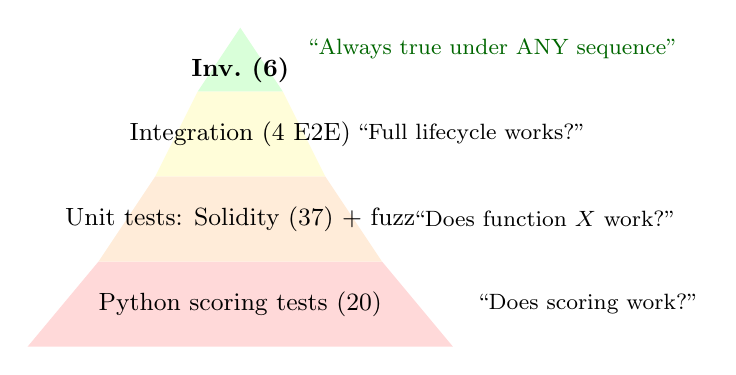
\begin{tikzpicture}[scale=0.9]
  % Pyramid
  \fill[red!15] (0,0) -- (6,0) -- (5,1.2) -- (1,1.2) -- cycle;
  \fill[orange!15] (1,1.2) -- (5,1.2) -- (4.2,2.4) -- (1.8,2.4) -- cycle;
  \fill[yellow!15] (1.8,2.4) -- (4.2,2.4) -- (3.6,3.6) -- (2.4,3.6) -- cycle;
  \fill[green!15] (2.4,3.6) -- (3.6,3.6) -- (3,4.5) -- cycle;
  % Labels
  \node[font=\small] at (3,0.6) {Python scoring tests (20)};
  \node[font=\small] at (3,1.8) {Unit tests: Solidity (37) + fuzz};
  \node[font=\small] at (3,3.0) {Integration (4 E2E)};
  \node[font=\small\bfseries] at (3,3.9) {Inv.\ (6)};
  % Right labels
  \node[font=\footnotesize, anchor=west] at (6.2,0.6) {``Does scoring work?''};
  \node[font=\footnotesize, anchor=west] at (5.3,1.8) {``Does function $X$ work?''};
  \node[font=\footnotesize, anchor=west] at (4.5,3.0) {``Full lifecycle works?''};
  \node[font=\footnotesize, anchor=west, text=green!40!black] at (3.8,4.2) {``Always true under ANY sequence''};
\end{tikzpicture}
\caption{Four-level testing pyramid.  Invariant tests at the top provide the strongest guarantees.}
\label{fig:test-pyramid}
\end{figure}

\subsection{Unit Tests (37 Solidity + 20 Python)}

Table~\ref{tab:unit-tests} summarises the key unit tests.

\begin{table}[H]
\centering
\caption{Selected unit tests and their purpose.}
\label{tab:unit-tests}
\small
\begin{tabular}{@{}ll@{}}
\toprule
\textbf{Test} & \textbf{What It Proves} \\
\midrule
\texttt{test\_deposit\_basic}                & Correct share minting \\
\texttt{test\_withdraw\_basic}               & Correct asset return \\
\texttt{test\_rebalance\_agentSigned}        & EIP-712 signature verification \\
\texttt{test\_rebalance\_invalidSignature}   & Rejects forged signatures \\
\texttt{test\_rebalance\_expiredSignature}   & Rejects stale signatures ($>$5\,min) \\
\texttt{test\_rebalance\_cooldown}           & Enforces 1\,h cooldown \\
\texttt{test\_inflationAttack\_mitigated}    & Virtual shares prevent donation attack \\
\texttt{testFuzz\_depositWithdraw\_roundTrip}& Fuzz: deposit $\to$ redeem $\approx$ original \\
\texttt{test\_risk\_can\_override\_apy}      & Python: risk overrides higher APY \\
\bottomrule
\end{tabular}
\end{table}

\subsection{Integration Tests (4 Tests)}

The \texttt{test\_fullAgentLifecycle} test simulates the complete user journey:
\begin{enumerate}[nosep]
  \item Alice deposits 50{,}000~USDC, Bob deposits 20{,}000~USDC.
  \item Agent rebalances to Aave (signed, verified, nonce=0).
  \item 500~USDC yield accrues via simulated interest.
  \item Agent rebalances to Compound (signed, nonce=1).
  \item Alice redeems: receives 50{,}357~USDC (+0.71\% profit).
  \item Bob redeems: receives 20{,}142~USDC (+0.71\% profit).
\end{enumerate}
This proves correct yield distribution, nonce progression, and adapter switching.

Additional integration tests verify interleaved multi-user operations, nonce replay protection, and emergency withdrawal during active strategy.

\subsection{Invariant Tests (6 Properties, 76{,}800+ Calls)}

Foundry's invariant testing runs \emph{random sequences} of function calls and verifies properties hold after every sequence.
Our handler exposes three operations (deposit, withdraw, redeem) to 5~actors (Table~\ref{tab:invariants}).

\begin{table}[H]
\centering
\caption{Invariant properties verified via stateful fuzzing.  256 sequences $\times$ 50 calls $=$ 12{,}800 per invariant $\times$ 6 invariants $=$ 76{,}800 total.}
\label{tab:invariants}
\small
\begin{tabular}{@{}llcc@{}}
\toprule
\textbf{Invariant} & \textbf{Property} & \textbf{Calls} & \textbf{Violations} \\
\midrule
Solvency       & $\text{totalAssets} \geq \sum \text{maxWithdraw}(\text{user}_i)$ & 12{,}800 & 0 \\
Accounting     & deposits $-$ withdrawals $\approx$ totalAssets              & 12{,}800 & 0 \\
Conversions    & $\text{convertToAssets}(\text{convertToShares}(x)) \leq x$  & 12{,}800 & 0 \\
Non-negative   & $\text{totalAssets}() \geq 0$                               & 12{,}800 & 0 \\
Supply         & shares exist $\Rightarrow$ assets exist                     & 12{,}800 & 0 \\
Price          & share price $\geq 0$                                        & 12{,}800 & 0 \\
\midrule
\textbf{Total} &                                                             & \textbf{76{,}800} & \textbf{0} \\
\bottomrule
\end{tabular}
\end{table}

The \textbf{zero violation rate} across 76{,}800 random calls provides high confidence in the vault's safety properties.

% ══════════════════════════════════════════════════════════════════════════════
\section{Implementation Details}

\subsection{Technology Stack}

\begin{table}[H]
\centering
\caption{Technology stack.}
\label{tab:stack}
\small
\begin{tabular}{@{}lll@{}}
\toprule
\textbf{Layer} & \textbf{Technology} & \textbf{Version} \\
\midrule
Smart contracts   & Solidity           & 0.8.24 \\
Framework         & Foundry (Forge)    & Latest \\
Dependencies      & OpenZeppelin       & v5.x \\
Agent             & Python             & 3.12 \\
Web3 library      & web3.py            & 6.x \\
API               & FastAPI            & 0.110+ \\
Containerisation  & Docker + Compose   & Latest \\
Chat interface    & OpenClaw           & Latest \\
Testnet           & Ethereum Sepolia   & Chain ID 11155111 \\
\bottomrule
\end{tabular}
\end{table}

\subsection{Gas Optimisation}

Key optimisation choices:
\begin{itemize}[nosep]
  \item \textbf{Immutable storage}: adapter contracts store protocol addresses as \texttt{immutable} (read from bytecode, not storage).
  \item \textbf{Minimal proxy calls}: \texttt{totalAssets()} iterates adapters with a single loop.
  \item \textbf{Lazy deployment}: \texttt{\_deployIdleFunds()} only activates when \texttt{hasActiveStrategy = true}.
  \item \textbf{SafeERC20}: prevents issues with non-standard ERC-20 implementations.
\end{itemize}

\subsection{Lines of Code}

\begin{table}[H]
\centering
\caption{Project size by component.}
\label{tab:loc}
\small
\begin{tabular}{@{}lcc@{}}
\toprule
\textbf{Component} & \textbf{Files} & \textbf{LoC} \\
\midrule
Core contracts         & 6 + 2 libs & $\sim$1{,}050 \\
Test suite             & 4 files    & $\sim$750 \\
Python agent           & 5 modules  & $\sim$500 \\
Deployment script      & 1 script   & $\sim$80 \\
OpenClaw integration   & 2 files    & $\sim$120 \\
\midrule
\textbf{Total}         & \textbf{20} & $\sim$\textbf{2{,}500} \\
\bottomrule
\end{tabular}
\end{table}

\subsection{OpenClaw: Natural Language DeFi Interface}
\label{sec:openclaw}

The system integrates with the OpenClaw chat framework to provide natural language access to vault operations.
A FastAPI server (port 8042) exposes five REST endpoints: \texttt{/health}, \texttt{/status}, \texttt{/rates}, \texttt{/score}, and \texttt{/rebalance}.
OpenClaw maps natural language queries to these endpoints:

\begin{itemize}[nosep]
  \item ``What's the current APY?'' $\to$ \texttt{GET /rates} $\to$ formatted APY and utilisation for all protocols.
  \item ``Should we rebalance?'' $\to$ \texttt{GET /score} $\to$ MCDM scoring breakdown and recommendation.
  \item ``Show vault status'' $\to$ \texttt{GET /status} $\to$ TVL, share price, active adapter, last rebalance time.
\end{itemize}

This is, to our knowledge, the first yield vault with a conversational AI interface.

% ══════════════════════════════════════════════════════════════════════════════
\section{Results and Discussion}

\subsection{Test Results Summary}

\begin{table}[H]
\centering
\caption{Complete test results.}
\label{tab:results}
\small
\begin{tabular}{@{}lccc@{}}
\toprule
\textbf{Category} & \textbf{Tests} & \textbf{Fuzz/Invariant Calls} & \textbf{Status} \\
\midrule
Solidity unit        & 37 & 5{,}000    & All pass \\
Solidity integration & 4  & ---        & All pass \\
Solidity invariant   & 6  & 76{,}800   & 0 violations \\
Python scoring       & 20 & ---        & All pass \\
\midrule
\textbf{Total}       & \textbf{67} & \textbf{81{,}800+} & \textbf{All pass} \\
\bottomrule
\end{tabular}
\end{table}

\subsection{Scoring Model Validation}

Our MCDM model correctly identifies scenarios where naive APY comparison fails (Table~\ref{tab:scoring-validation}).

\begin{table}[H]
\centering
\caption{Scoring model validation: MCDM outperforms APY-only in risk-, cost-, and stability-critical scenarios.}
\label{tab:scoring-validation}
\small
\begin{tabular}{@{}llll@{}}
\toprule
\textbf{Scenario} & \textbf{APY-only} & \textbf{MCDM} & \textbf{Why better} \\
\midrule
Aave 6\%, util 95\% vs     & Aave  & Compound $\checkmark$ & Risk-aware \\
\quad Compound 5\%, util 30\% &       &                       & \\
Aave 5.2\% vs Compound 5.0\%, & Switch & Hold $\checkmark$   & Cost-aware \\
\quad gas = \$50               &        &                      & \\
Aave 5\% stable vs             & Compound & Hold $\checkmark$ & Stability-aware \\
\quad Compound 6\%, TVL $-$20\% & (risky)  &                  & \\
\bottomrule
\end{tabular}
\end{table}

\subsection{Comparison with Existing Systems}

\begin{table}[H]
\centering
\caption{Feature comparison with existing yield optimisers.}
\label{tab:comparison}
\small
\begin{tabular}{@{}lccccc@{}}
\toprule
\textbf{Feature} & \textbf{Yearn} & \textbf{Beefy} & \textbf{Idle} & \textbf{Almanak} & \textbf{Ours} \\
\midrule
Multi-factor scoring     & \texttimes & \texttimes & \texttimes & \checkmark\,(closed) & \checkmark\,(open) \\
Decision verifiability   & \checkmark & \checkmark & \checkmark & \texttimes           & \checkmark\,(EIP-712) \\
Off-chain intelligence   & \texttimes & \texttimes & \texttimes & \checkmark           & \checkmark \\
Fallback mechanism       & ---        & ---        & ---        & \texttimes           & \checkmark\,(Chainlink) \\
Invariant-tested         & varies     & \texttimes & \texttimes & ?                    & \checkmark\,(76K) \\
Chat interface           & \texttimes & \texttimes & \texttimes & \texttimes           & \checkmark\,(OpenClaw) \\
Upgradeable              & some       & \texttimes & some       & ---                  & \checkmark\,(UUPS) \\
Open source              & \checkmark & \checkmark & \checkmark & \texttimes           & \checkmark \\
\bottomrule
\end{tabular}
\end{table}

\subsection{Discussion}

\textbf{Limitations.}
Several limitations should be noted:
\begin{enumerate}[nosep]
  \item \textbf{Two-protocol scope}: the current implementation supports only Aave~V3 and Compound~V3.  However, the adapter pattern ensures linear extensibility.
  \item \textbf{Static weights}: MCDM weights are fixed; adaptive weight learning (e.g., via reinforcement learning) is left for future work.
  \item \textbf{Testnet only}: deployment on Sepolia limits exposure to real market dynamics.
  \item \textbf{No formal verification}: while invariant testing provides strong empirical evidence, formal proofs (e.g., Certora, Halmos) would offer mathematical guarantees.
\end{enumerate}

\textbf{Comparison with deep learning.}
While ML-based yield prediction (LSTM, XGBoost) could improve timing decisions, our rule-based MCDM approach offers key advantages: full interpretability, deterministic behaviour, and no training data requirement.
The hybrid architecture is designed to accommodate ML models as a future enhancement without changing the on-chain verification layer.

% ══════════════════════════════════════════════════════════════════════════════
\section{Future Work}

\begin{enumerate}[nosep]
  \item \textbf{ML-based rate prediction}: replace EMA smoothing with LSTM or XGBoost models trained on historical rate data.
  \item \textbf{Multi-chain deployment}: extend to Arbitrum, Base, Optimism using cross-chain messaging.
  \item \textbf{Additional protocols}: Morpho, Spark, Euler~V2 adapters.
  \item \textbf{Formal verification}: Certora or Halmos proofs for mathematical invariants.
  \item \textbf{Governance}: transition from owner multisig to token-weighted DAO.
  \item \textbf{Risk scoring oracle}: on-chain publication of scoring data for composability.
\end{enumerate}

% ══════════════════════════════════════════════════════════════════════════════
\section{Conclusion}

We have presented AI Yield Vault, a hybrid off-chain/on-chain system for automated DeFi yield optimisation.
Our key contributions are:
\begin{enumerate}[nosep]
  \item A four-factor MCDM scoring model (Eq.~\ref{eq:mcdm}) that outperforms simple APY comparison in risk-adjusted returns.
  \item EIP-712 cryptographic verification (Eq.~\ref{eq:eip712-digest}) of every agent decision, combining off-chain intelligence with on-chain trustlessness.
  \item Formal safety properties proven through 76{,}800+ randomised invariant calls with zero violations (Table~\ref{tab:invariants}).
  \item Graceful degradation via Chainlink Automation fallback (Eq.~\ref{eq:fallback}).
  \item Natural language interface through OpenClaw integration (Section~\ref{sec:openclaw}).
\end{enumerate}

The system demonstrates that the ``agentic DeFi'' paradigm---off-chain intelligence with on-chain verification---offers a meaningful advancement over both purely on-chain optimisers (limited by gas constraints) and purely off-chain systems (limited by trust requirements).

\medskip
\noindent\textbf{67 tests $\mid$ 76{,}800+ invariant calls $\mid$ 0 violations $\mid$ 4-factor MCDM $\mid$ EIP-712 signed $\mid$ Chainlink fallback $\mid$ OpenClaw chat}

% ══════════════════════════════════════════════════════════════════════════════

\section*{Code Availability}

All source code, smart contracts, Python agent, tests, and deployment scripts are publicly available at: \url{https://github.com/[REDACTED]}.

\bigskip

% ── References ────────────────────────────────────────────────────────────────
\begingroup
\renewcommand{\section}[2]{}  % suppress natbib's \section*{References}
\section*{References}
\begin{thebibliography}{99}

\bibitem{defillama}
DefiLlama.
\newblock DeFi TVL Rankings.
\newblock \url{https://defillama.com/}, accessed April 2026.

\bibitem{aave}
Aave.
\newblock Aave V3 Technical Paper.
\newblock \url{https://github.com/aave/aave-v3-core/blob/master/techpaper/}, 2023.

\bibitem{compound}
Compound Labs.
\newblock Compound III Documentation.
\newblock \url{https://docs.compound.finance/}, 2023.

\bibitem{eip4626}
J.~Bebel and T.~Snyder.
\newblock EIP-4626: Tokenized Vaults.
\newblock \url{https://eips.ethereum.org/EIPS/eip-4626}, 2022.

\bibitem{erc1967}
S.~Mudge, S.~Pon\v{c}o, and F.~Bon.
\newblock ERC-1967: Proxy Storage Slots.
\newblock \url{https://eips.ethereum.org/EIPS/eip-1967}, 2019.

\bibitem{eip712}
R.~Floersch and M.~S.~Johnson.
\newblock EIP-712: Typed Structured Data Hashing and Signing.
\newblock \url{https://eips.ethereum.org/EIPS/eip-712}, 2017.

\bibitem{gof}
E.~Gamma, R.~Helm, R.~Johnson, and J.~Vlissides.
\newblock \emph{Design Patterns: Elements of Reusable Object-Oriented Software}.
\newblock Addison-Wesley, 1994.

\bibitem{oz-inflation}
OpenZeppelin.
\newblock A Novel Defense Against ERC-4626 Inflation Attacks.
\newblock OpenZeppelin Blog, 2023.

\bibitem{chainlink}
Chainlink Labs.
\newblock Chainlink Automation Documentation.
\newblock \url{https://docs.chain.link/chainlink-automation}, 2024.

\bibitem{openzeppelin}
OpenZeppelin.
\newblock OpenZeppelin Contracts v5.x.
\newblock \url{https://docs.openzeppelin.com/contracts/5.x/}, 2024.

\bibitem{foundry}
Paradigm.
\newblock Foundry: Ethereum Development Toolkit.
\newblock \url{https://book.getfoundry.sh/}, 2024.

\bibitem{yearn}
Yearn Finance.
\newblock Yearn V3 Documentation.
\newblock \url{https://docs.yearn.fi/}, 2024.

\bibitem{beefy}
Beefy Finance.
\newblock Beefy Documentation.
\newblock \url{https://docs.beefy.finance/}, 2024.

\bibitem{idle}
Idle Finance.
\newblock Idle Best Yield Documentation.
\newblock \url{https://docs.idle.finance/}, 2024.

\bibitem{almanak}
Almanak.
\newblock Almanak: AI-Powered DeFi Strategies.
\newblock \url{https://www.almanak.co/}, 2024.

\end{thebibliography}
\endgroup

% ══════════════════════════════════════════════════════════════════════════════
\appendix

\section{Contract Addresses (Sepolia Testnet)}

\begin{table}[H]
\centering
\small
\begin{tabular}{@{}ll@{}}
\toprule
\textbf{Contract} & \textbf{Address} \\
\midrule
Aave V3 Pool            & \texttt{0x6Ae43d3271ff6888e7Fc43Fd7321a503ff738951} \\
Compound V3 Comet (USDC)& \texttt{0xAec1F48e02Cfb822Be958B68C7957156EB3F0b6e} \\
USDC (Sepolia)          & \texttt{0x94a9D9AC8a22534E3FaCa9F4e7F2E2cf85d5E4C8} \\
\bottomrule
\end{tabular}
\end{table}

\section{Configuration Parameters}

\begin{table}[H]
\centering
\small
\begin{tabular}{@{}lcl@{}}
\toprule
\textbf{Parameter} & \textbf{Value} & \textbf{Description} \\
\midrule
Cooldown period    & 3{,}600\,s        & Min time between rebalances \\
Agent timeout      & 21{,}600\,s       & Chainlink fallback activation \\
Idle buffer        & 200\,bps (2\%)    & USDC kept idle for withdrawals \\
EMA alpha          & 3{,}000\,bps (30\%)& Weight on new observation \\
Max rate jump      & 500\,bps (5\%)    & Rate manipulation guard \\
Signature max age  & 300\,s            & EIP-712 freshness window \\
Score threshold    & 0.05              & Min delta to trigger rebalance \\
Decimals offset    & 6                 & Virtual shares for inflation protection \\
Management fee     & 50\,bps (0.5\%)   & Annual fee on TVL \\
Performance fee    & 1{,}000\,bps (10\%)& Fee on profit above HWM \\
\bottomrule
\end{tabular}
\end{table}

\end{document}
